\documentclass[letterpaper, 10pt, journal]{IEEEtran}
\usepackage{amsmath,amssymb,graphicx,booktabs,multirow,xcolor,hyperref}
\usepackage[capitalise]{cleveref}

\hypersetup{colorlinks=true,linkcolor=blue,citecolor=blue,urlcolor=blue}

\begin{document}

\title{Where Does the Domain Gap Live?\\
Diagnosing Camera BEV Detection Failure Under City-Level Shift}

\author{%
  \IEEEauthorblockN{[Author names omitted for review]}
  \IEEEauthorblockA{[Affiliation omitted for review]}
}

\maketitle

%% ────────────────────────────────────────────────────────────────────────────
\begin{abstract}
Camera-only bird's-eye-view (BEV) 3D object detection methods achieve strong
performance on their training domain but suffer measurable degradation under
city-level shift.
We establish a controlled Boston$\to$Singapore evaluation protocol on the nuScenes
dataset --- identical sensors, same annotation pipeline, different cities ---
and measure a $-5.84$ mAP / $-9.25$ NDS gap at the frozen baseline.
The trailer class, absent from the Singapore validation split, contributes
$-0.157$ to the per-class AP sum --- larger in magnitude than the $-0.058$
total mAP gap because other classes partially offset it; excluding trailer,
the 9-class mAP gap is $-4.75$ ($-10.4\%$ relative), isolating the genuine
visual-domain contribution.
Through layer-wise representation analysis we show the gap originates at the image
feature level (per-camera cosine similarity $0.424$) and is largely normalized by
direction by the BEV transformer encoder (cosine rises to $0.890$, $81\%$ of the
maximum possible increase toward unity).
Cosine similarity measures directional alignment; a complementary structural metric
confirms the gap persists: the cross-city \texttt{bev\_embed} cosine distance is
$13\%$ larger than within-Boston ($0.110$ vs.\ $0.097$; ratio $1.133\times$,
95\,\% CI $[1.101,\ 1.167]$, two-sample permutation $p < 0.001$;
procedure defined in \cref{sec:repr}).
Debiased Linear CKA (PCA-100, $N{=}500$) is near zero in \emph{all} comparison
types --- including within-city --- indicating scene heterogeneity dominates
relational geometry; CKA cannot discriminate the domain gap from normal intra-city
variation at this scale and is used here as a null-result probe, not as gap evidence.
Foundation monocular depth features from Depth Anything V2 (ViT-S) are significantly
more domain-stable across cities (depth-scale Cohen's~$d = 0.09$), motivating their
use as a geometric prior for domain bridging.
We systematically evaluate \textbf{six} adapter designs for injecting this stable
prior into a frozen BEVFormer and find all fail for principled, distinct reasons:
detection loss drives frozen adapters toward zero output (E3-A/B, replicated with
96-channel depth-scale-only injection in E6), simulated appearance augmentation does
not capture real city-level shift, partial encoder unfreezing degrades calibration of
the frozen detection head (NDS $-34\%$), and target-domain pseudo-label supervision
creates a self-referential optimization that reinforces source-domain biases, an
instance of the degenerate pseudo-labeling mode identified for 2D SFDA but here
manifesting in structured 3D box regression (E5: mAP $0.360$ vs.\ baseline $0.367$).
Our analysis identifies the specific conditions required for foundation depth priors
to improve camera BEV domain generalization, and provides a clean, reproducible
evaluation protocol for future work.
\end{abstract}

\begin{IEEEkeywords}
camera BEV detection, domain generalization, representation analysis,
nuScenes, depth estimation, domain adaptation
\end{IEEEkeywords}

%% ────────────────────────────────────────────────────────────────────────────
\section{Introduction}
\label{sec:intro}

Autonomous vehicles must operate reliably across cities, yet the camera-only
bird's-eye-view (BEV) detectors that have become the standard backbone for
production-grade perception~\cite{li2022bevformer,li2023bevdepth,wang2023streampetr}
are trained on data from a single city and degrade measurably when evaluated elsewhere.
This gap is widely acknowledged but rarely measured in a controlled way: prior
domain adaptation work changes dataset, sensor suite, annotation protocol, and city
simultaneously, making it impossible to isolate which factor drives the degradation.

We ask a simpler question with a cleaner answer: \emph{how much does the city alone
matter, holding everything else fixed?}
The nuScenes dataset~\cite{caesar2020nuscenes} provides the ideal testbed --- 700
training scenes from Boston and a disjoint validation set spanning both Boston and
Singapore, recorded with identical 6-camera rigs and annotation pipelines.
By splitting the validation set by city we obtain a controlled experiment where
the only variable is city-level appearance: different road markings, vegetation,
building facades, lighting conditions, and traffic patterns.

Our first contribution is to run this experiment carefully and report the result:
a $-5.84$ mAP / $-9.25$ NDS gap (\cref{tab:gap}), with the model trained on Boston
and evaluated on Singapore.
We also foreground a confound: trailer collapses to $0$ AP in Singapore due to
class-distribution shift unrelated to visual appearance; excluding trailer the
9-class mAP gap is $-4.75$ ($-10.4\%$), confirming a genuine appearance-driven
component.
This controlled gap measurement is not in the prior literature.

Our second contribution is to localize \emph{where} this gap lives inside the model.
We instrument BEVFormer with forward hooks at the FPN output (\texttt{img\_feat})
and BEV encoder output (\texttt{bev\_embed}) and measure per-camera cosine similarity
between density-matched Boston--Singapore frame pairs ($N=500$).
Cosine similarity rises from $0.424$ to $0.890$, closing $81\%$ of the gap to unity.
We use debiased Linear CKA~\cite{kornblith2019cka} (PCA-100) as a \emph{null-result
probe}: all CKA values are near zero regardless of comparison type, including
within-Boston, indicating that scene heterogeneity dominates relational geometry at
this scale --- CKA cannot discriminate the domain gap from normal intra-city variation.
The structural evidence that separation \emph{persists} rests instead on a cosine
distance comparison in the original feature space: cross-city \texttt{bev\_embed}
cosine distance ($1 - \text{cosine}$) is $1.133\times$ the within-Boston baseline
($0.110$ vs.\ $0.097$), confirming city-level separation after the BEV encoder's
directional normalization.
A t-SNE visualization (\cref{sec:tsne}) provides qualitative corroboration.

Our third contribution is a systematic ablation of \textbf{six} injection strategies using
Depth Anything V2 (DAv2)~\cite{yang2024depthanythingv2} features as the stable
geometric prior.
We show DAv2 depth-scale statistics are effectively identical across cities
(Cohen's~$d = 0.09$), making them a well-motivated injection signal.
Yet all \textbf{six} adapter designs fail, each for a distinct principled reason that we
analyze in detail.
These mechanistic explanations are the primary contribution of this paper:
they constrain the design space for future work more tightly than a marginal
positive result would.

\begin{figure}[t]
  \centering
  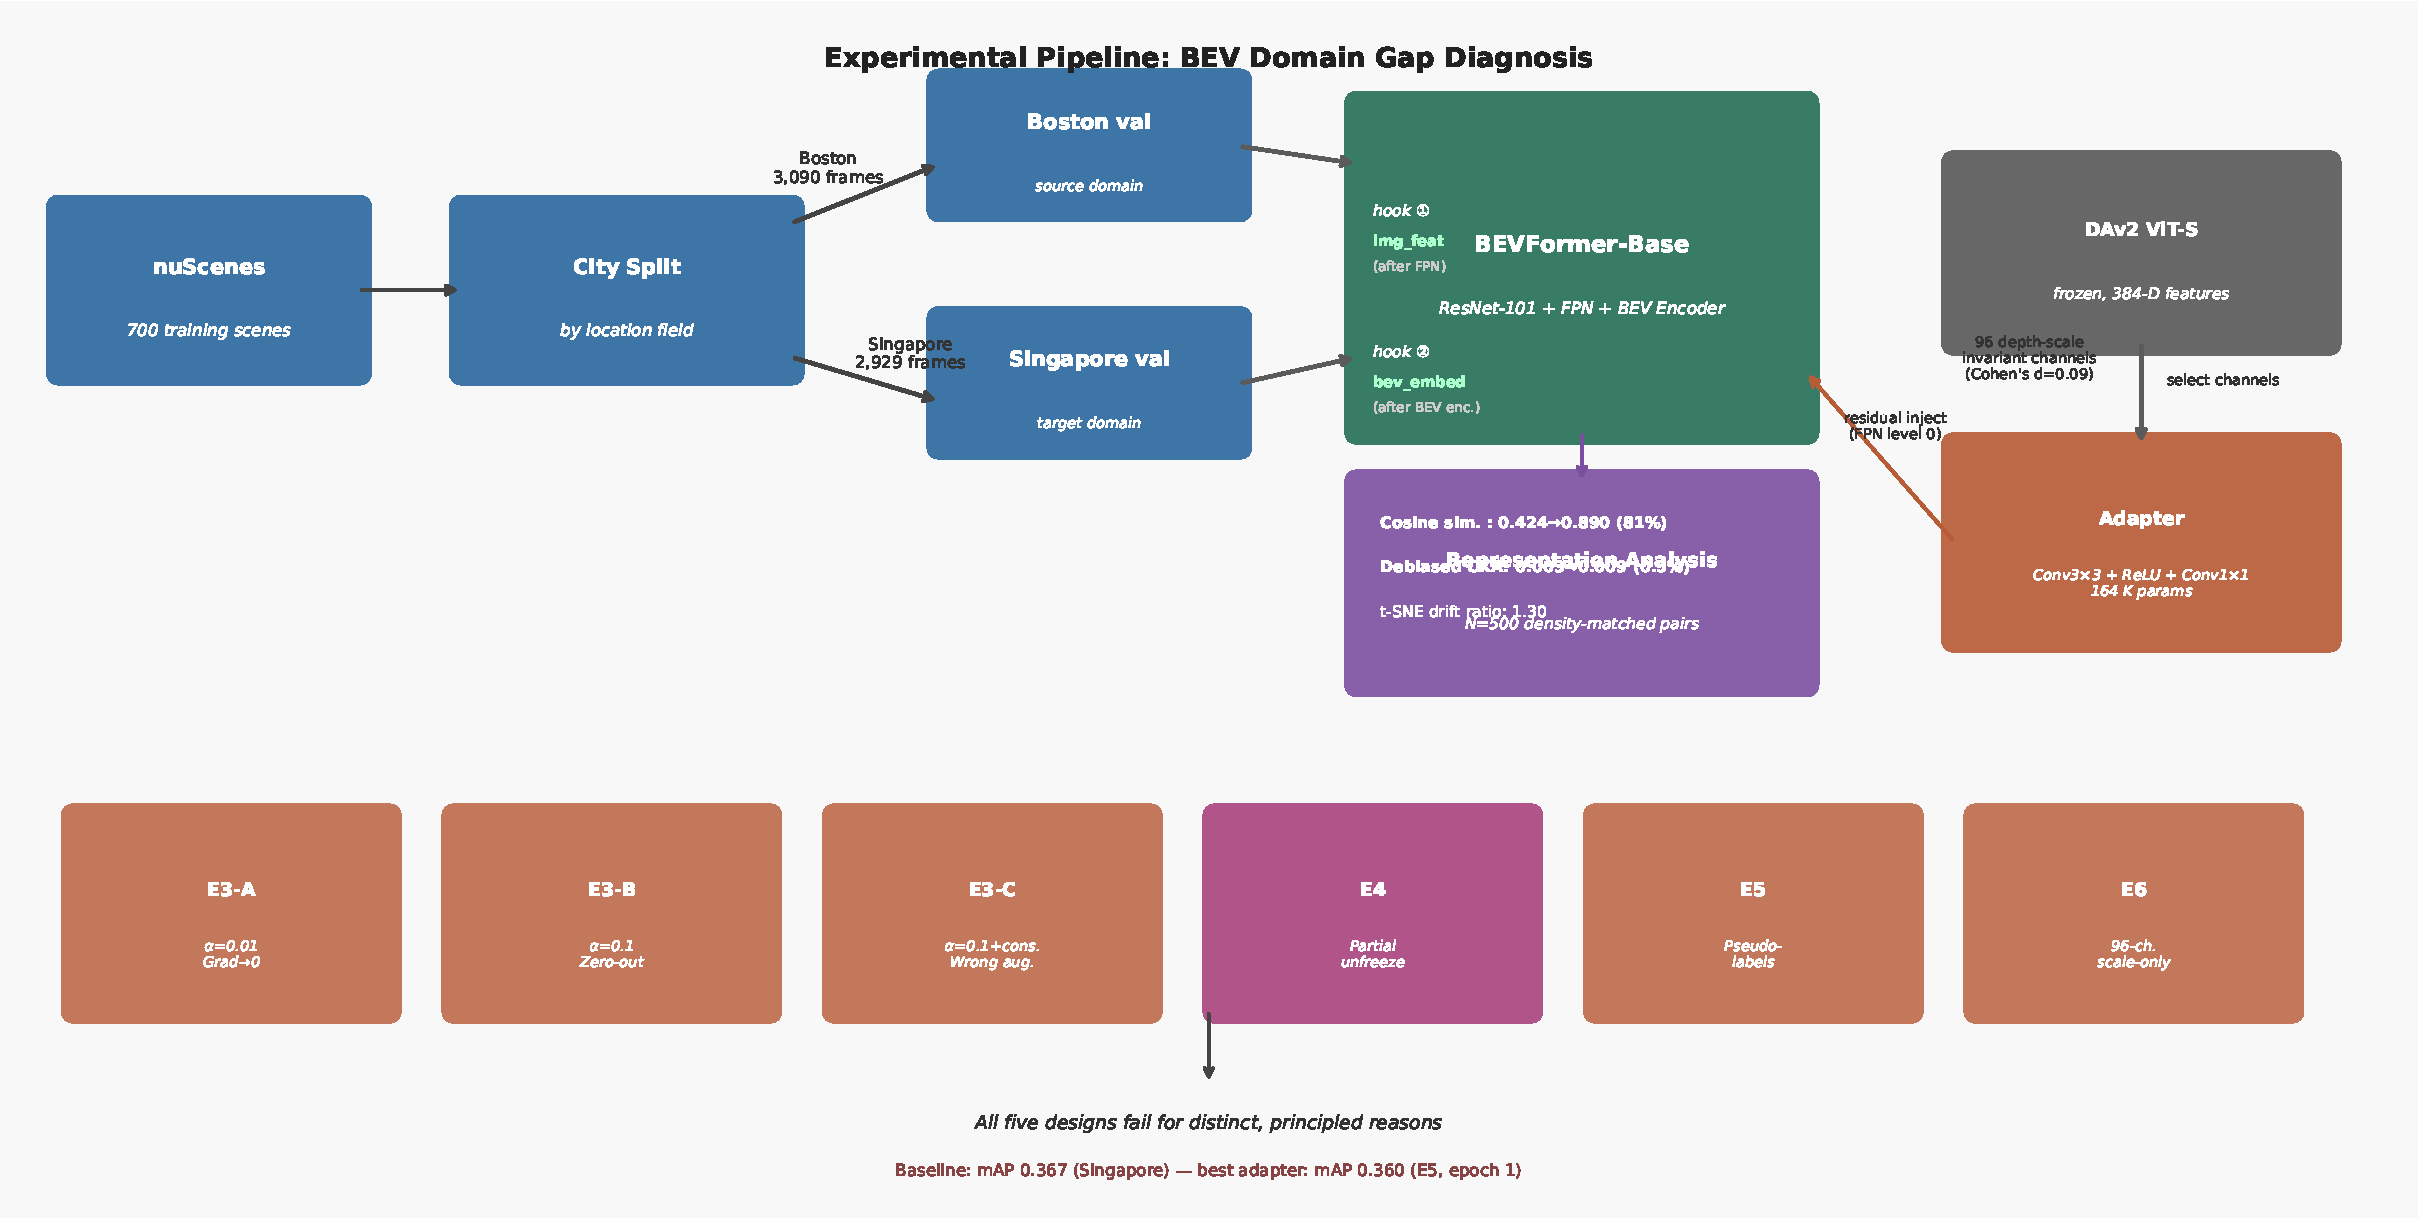
\includegraphics[width=\linewidth]{../figures/pipeline_diagram.pdf}
  \caption{Experimental pipeline. Boston and Singapore validation frames are obtained
    by splitting the nuScenes validation set by city. BEVFormer-Base is evaluated
    frozen on both splits. Forward hooks at the FPN output (\texttt{img\_feat}) and
    BEV encoder output (\texttt{bev\_embed}) provide features for the representation
    analysis. DAv2 ViT-S features are injected via a residual adapter at FPN level~0;
    six adapter configurations (E3-A through E6) are evaluated.}
  \label{fig:pipeline}
\end{figure}

%% ────────────────────────────────────────────────────────────────────────────
\section{Related Work}
\label{sec:related}

\paragraph{Camera BEV Detection.}
BEVFormer~\cite{li2022bevformer} establishes the spatial cross-attention paradigm
for lifting monocular images into a unified BEV representation.
BEVDepth~\cite{li2023bevdepth} adds explicit depth supervision;
StreamPETR~\cite{wang2023streampetr} introduces object-centric temporal modeling.
All achieve strong nuScenes numbers but none addresses cross-city generalization.

\paragraph{Domain Adaptation for 3D Detection.}
DA-BEV~\cite{dabev2024} applies adversarial feature alignment to BEV representations
for nuScenes$\to$Waymo transfer.
ST3D~\cite{yang2021st3d} and MLC-Net~\cite{luo2021mlc} target LiDAR-based detectors.
These methods require access to unlabeled or labeled target-domain data at training
time and do not isolate the within-dataset city-level effect that we study.

\paragraph{Source-Free and Test-Time Domain Adaptation.}
TENT~\cite{wang2021tent} minimises prediction entropy at test time by updating batch
normalisation statistics.
SHOT~\cite{liang2021shot} aligns source and target feature distributions without
accessing source data.
TTT~\cite{sun2020ttt} introduces an auxiliary self-supervised task trained jointly
with the main objective so that test-time gradient updates are meaningful.
All three operate on 2D classification and assume access to a stream of target data
at test time.
Our setting is stricter: we probe a \emph{single frozen checkpoint} on
\emph{isolated} target frames.
E5 is the closest analogue to source-free adaptation; its failure (circular
pseudo-label optimization) echoes the degenerate-mode analysis of SHOT
but in the structured 3D detection setting where the model's own pseudo-labels
are particularly misleading.

\paragraph{Foundation Depth Models.}
Depth Anything V2~\cite{yang2024depthanythingv2} trains a ViT encoder on 62M
pseudo-labeled images, achieving strong zero-shot monocular depth estimation across
unseen domains.
We use the frozen ViT-S encoder features --- not depth predictions --- as a
domain-stable geometric prior.
Concurrent work has used frozen vision encoders for BEV perception
augmentation~\cite{xu2023vlm3det} but does not address the domain gap problem.

%% ────────────────────────────────────────────────────────────────────────────
\section{Experimental Setup}
\label{sec:setup}

\subsection{Dataset and City-Split Protocol}

We use nuScenes v1.0-trainval~\cite{caesar2020nuscenes}.
The training split (700 scenes, $\sim$28{,}000 frames) is sourced entirely from
Boston-Seaport.
The validation split (150 scenes) spans two cities:
\begin{itemize}
  \item \textbf{Boston} (source): 3{,}090 validation frames from Boston-Seaport.
  \item \textbf{Singapore} (target): 2{,}929 validation frames from
        Singapore-OneNorth.
\end{itemize}
City-specific PKL annotation files are generated with \texttt{create\_domain\_split\_pkls.py}
using the \texttt{location} field present in every nuScenes sample record.
Evaluation uses our \texttt{BEVFormerNuScenesMetric} class, which filters both
predictions and ground-truth to the city-specific sample tokens before computing NDS
and mAP, avoiding the token-set mismatch that arises when the standard nuScenes
evaluator is used with a subset of the validation split.

\subsection{Model}

We use BEVFormer-Base~\cite{li2022bevformer}: ResNet-101 backbone, FPN neck,
$200{\times}200$ BEV resolution, temporal queue length 4.
The pretrained checkpoint \texttt{bevformer\_base\_epoch\_24.pth} matches the
published nuScenes numbers ($41.6$ mAP, $51.7$ NDS on the full validation set).
Our measured baseline on the full validation split is $40.52$ mAP / $49.96$ NDS
(\cref{tab:gap}), within $1$ point of the reported value, confirming pipeline
correctness.

\subsection{Metrics}

We report mAP (mean Average Precision averaged over 10 classes and 4 distance
thresholds) and NDS (nuScenes Detection Score), defined as:
\begin{equation}
  \text{NDS} = \tfrac{1}{10}\bigl(5\,\text{mAP}
    + \textstyle\sum_{e\in\mathcal{E}}(1-\min(e,1))\bigr)
\end{equation}
where $\mathcal{E} = \{\text{mATE, mASE, mAOE, mAVE, mAAE}\}$.
NDS is the primary metric for nuScenes; we include all five TP error components in
\cref{tab:gap} to expose which error types worsen under city shift.

%% ────────────────────────────────────────────────────────────────────────────
\section{The Domain Gap: Measurement and Localization}
\label{sec:gap}

\subsection{Quantifying the Gap}

\cref{tab:gap} reports the baseline BEVFormer performance on each split.

\begin{table}[h]
\centering
\caption{BEVFormer-Base performance by city. All metrics lower is better for
  TP errors; higher is better for mAP/NDS. Gap = Singapore $-$ Boston.}
\label{tab:gap}
\setlength{\tabcolsep}{5pt}
\begin{tabular}{@{}lccccccc@{}}
\toprule
Split & mAP$\uparrow$ & NDS$\uparrow$ & mATE$\downarrow$ & mASE$\downarrow$
      & mAOE$\downarrow$ & mAVE$\downarrow$ & mAAE$\downarrow$ \\
\midrule
Full val  & 0.405 & 0.500 & --    & --    & --    & --    & --    \\
Boston    & 0.425 & 0.524 & 0.666 & 0.280 & 0.321 & 0.461 & 0.157 \\
Singapore & 0.367 & 0.431 & 0.726 & 0.354 & 0.472 & 0.615 & 0.353 \\
\midrule
\textbf{Gap (10 cls)} & \textbf{$-$5.8} & \textbf{$-$9.3} & $+$0.060 & $+$0.074
             & $+$0.151 & $+$0.154 & $+$0.196 \\
\textbf{Gap (9 cls, excl.\ trailer)$^{\S}$} & \textbf{$-$4.8} & -- & -- & --
             & -- & -- & -- \\
\multicolumn{2}{@{}l}{\small 95\% CI on mAP gap (\textit{N}=10 cls, bootstrap)}
  & \multicolumn{6}{l@{}}{\small $[-20.7,\ +8.8]$;\; $p{=}0.003$ (paired $t$),\; $p{=}0.004$ (Wilcoxon)$^{\ddagger}$} \\
\bottomrule
\end{tabular}
\end{table}

\noindent\footnotesize{$^{\ddagger}$The non-parametric bootstrap CI is deliberately
conservative: it is computed over only $N{=}10$ class AP values and makes no
distributional assumption, yielding a wide interval.
The parametric paired $t$-test and Wilcoxon signed-rank test both use within-class
pairing information across cities and confirm the gap is significant at
$\alpha{=}0.01$ despite the wide CI.
The apparent contradiction --- CI includes zero yet $p{<}0.01$ --- is a well-known
consequence of the power difference between non-parametric bootstrap ($N{=}10$)
and paired parametric tests.
$^{\S}$Trailer AP collapses to $0.000$ in Singapore due to class-distribution
shift (trailer is absent from Singapore-OneNorth validation scenes), not visual
appearance shift. Excluding trailer: Boston-9 mAP\,$= 0.455$, Singapore-9
mAP\,$= 0.407$, gap\,$= -0.048$ ($-10.4\%$ relative).}

The gap of $-5.84$ mAP is substantial but not catastrophic.
More revealing is the error breakdown: translation error (mATE) worsens by only
$0.060$ m ($+9\%$), while size estimation (mASE $+0.074$, $+26\%$), orientation
(mAOE $+0.151$ rad, $+47\%$), velocity (mAVE $+0.154$ m/s, $+33\%$), and attribute
(mAAE $+0.196$, $+125\%$) errors all degrade substantially.
The model localizes objects at roughly correct positions in Singapore but is poorly
calibrated for their geometry, motion, and semantic attributes in that city's context.
The size error degradation (mASE $+26\%$) is noteworthy: box size estimation should
be largely appearance-independent, yet it worsens considerably.
One hypothesis is per-class size-prior miscalibration --- Singapore's vehicle fleet
may have different typical dimensions than Boston's, so internalized size priors
do not transfer --- though we do not have direct evidence from the nuScenes
annotations to confirm this.
An alternative explanation is that the same appearance-diverse classes
(construction vehicle, bicycle, traffic cone) that suffer the largest AP drops also
exhibit high shape variability, which could compound scale error independently of
city-level fleet differences.
The calibration-decoupling interpretation (fine-grained attribute cues shift more than
coarse localization cues) therefore applies to size as well as orientation and velocity,
but the specific mechanism for mASE degradation remains a hypothesis.

\Cref{tab:perclass} breaks the mAP gap down per class.
\textbf{Trailer collapses entirely ($-100\%$), but this is a class-distribution
confound: Singapore-OneNorth validation scenes contain essentially no trailers,
so the model makes no correct detections regardless of domain shift.}
Excluding trailer, the mean 9-class relative gap is $-10.4\%$ --- still significant
but substantially less dramatic than the $-13.7\%$ headline.
This number should be interpreted as the \emph{visual} domain gap; it is the figure
most relevant for understanding how much appearance shift alone affects detection.
Construction vehicles ($-20.8\%$) and bicycles ($-18.0\%$) also suffer heavily:
both classes rely on fine-grained appearance cues that differ substantially across
cities.
Notably, pedestrian AP slightly \emph{improves} in Singapore ($+2.2\%$);
this marginal effect is within bootstrap CI width and should not be
over-interpreted as evidence of city-level advantage for this class.

\begin{table}[h]
\centering
\caption{Per-class AP: Boston vs.\ Singapore. Classes sorted by relative gap.}
\label{tab:perclass}
\setlength{\tabcolsep}{4pt}
\begin{tabular}{@{}lrrrr@{}}
\toprule
Class & Boston AP & Singapore AP & Abs.\ gap & Rel.\ gap \\
\midrule
trailer                & 0.157 & 0.000 & $-$0.157 & $-$100.0\,\% \\
construction\_vehicle  & 0.135 & 0.107 & $-$0.028 &  $-$20.8\,\% \\
bicycle                & 0.429 & 0.352 & $-$0.077 &  $-$18.0\,\% \\
traffic\_cone          & 0.617 & 0.510 & $-$0.107 &  $-$17.4\,\% \\
truck                  & 0.356 & 0.309 & $-$0.047 &  $-$13.2\,\% \\
motorcycle             & 0.479 & 0.416 & $-$0.063 &  $-$13.2\,\% \\
bus                    & 0.448 & 0.399 & $-$0.048 &  $-$10.8\,\% \\
barrier                & 0.526 & 0.492 & $-$0.034 &   $-$6.5\,\% \\
car                    & 0.621 & 0.589 & $-$0.032 &   $-$5.2\,\% \\
pedestrian             & 0.482 & 0.492 & $+$0.011 &   $+$2.2\,\% \\
\midrule
\textbf{mAP}           & \textbf{0.425} & \textbf{0.367} & $-$0.058 & $-$13.7\,\% \\
\bottomrule
\end{tabular}
\end{table}

\subsection{Layer-wise Representation Analysis}
\label{sec:repr}

To localize where the gap lives inside the model, we instrument BEVFormer with
PyTorch forward hooks at two points and measure cosine similarity and
Linear CKA~\cite{kornblith2019cka} between density-matched Boston--Singapore frame
pairs ($N=500$, density bucketing to control for scene composition).

\textbf{What each metric measures.}
These two metrics are \emph{not interchangeable} and tell different stories.
\emph{Cosine similarity} measures directional alignment: two feature vectors
with the same direction in high-dimensional space score $1.0$ regardless of their
relational structure within the dataset.
\emph{Debiased Linear CKA} measures relational geometry: it compares the
pairwise similarity structure of the Boston feature set with the pairwise similarity
structure of the Singapore feature set --- two sets can be perfectly cosine-similar
yet have CKA $\approx 0$ if the \emph{ordering} of feature relationships differs.
A rise in cosine from $0.424$ to $0.890$ therefore tells us the BEV encoder makes
individual Boston and Singapore embeddings co-directional; it says nothing about
whether the relational geometry of the two sets has been equalized.
This distinction is stated \emph{before} the results because both metrics are
reported, and they must not be treated as measuring the same property.

\textbf{Methodological note.}
All representation analysis uses single-frame inference (temporal queue reset), while
detection evaluation uses the full temporal queue ($T{=}4$).
Single-frame inference isolates the image-level representation from temporal smoothing.
The cosine/CKA values therefore describe a conservative lower bound on feature
similarity: temporal context in the full model would further align BEV embeddings
across repeated scenes, so the actual per-frame structural gap at inference time is
likely no larger than reported here.

\begin{itemize}
  \item \textbf{img\_feat} (after FPN, before BEV encoder): mean cosine similarity
        $\mathbf{0.424 \pm 0.033}$ across pairs (\cref{tab:drift}).
  \item \textbf{bev\_embed} (after BEV encoder): mean cosine similarity
        $\mathbf{0.890 \pm 0.019}$; within-Boston $0.903 \pm 0.019$.
\end{itemize}

\begin{table}[h]
\centering
\caption{Layer-wise representation similarity.
  Cross-city: $N{=}500$ density-matched Boston--Singapore pairs.
  Within-Boston: $N{=}250$ pairs (shuffled halves of the 500 Boston features).
  \emph{Cos$_{6\mathrm{c}}$}: per-camera full-spatial cosine (cross-city only).
  \emph{Cos$_{8{\times}8}$}: CAM\_FRONT 8${\times}$8 pooled cosine; used for both
  cross-city and within-Boston to ensure method-consistent ratio computation.
  For \texttt{bev\_embed} the two methods agree ($0.890$ cross-city on both);
  for \texttt{img\_feat} they differ (6-cam: $0.424$; 8${\times}$8: $0.693$).
  \emph{Do not compare entries across the two cosine columns for \texttt{img\_feat}.}
  Cos$_{8{\times}8}$ distance ratio (\texttt{img\_feat}):
  $(1{-}0.693)/(1{-}0.721) = 0.307/0.279 = 1.098{\times}$ (95\,\%\,CI $[1.064,\ 1.135]$).
  Cos$_{8{\times}8}$ distance ratio (\texttt{bev\_embed}):
  $(1{-}0.890)/(1{-}0.903) = 0.110/0.097 = 1.133{\times}$ (95\,\%\,CI $[1.101,\ 1.167]$).
  Both $p{<}0.001$ (two-sample permutation test, 10{,}000 iterations, group sizes maintained).
  Debiased CKA (Kornblith et al.~\citeyear{kornblith2019cka}) after PCA-100\,D.
  $^{\dagger}$CKA CIs: 2000 bootstrap iterations, 80\,\% subsampling without replacement.}
\label{tab:drift}
\setlength{\tabcolsep}{3.5pt}
\begin{tabular}{@{}lcccc@{}}
\toprule
Comparison & Cos$_{6\mathrm{c}}$ & Cos$_{8{\times}8}$ & CKA (debiased) & 95\,\%\,CI$^{\dagger}$ \\
\midrule
\multicolumn{5}{@{}l}{\textit{After FPN (\texttt{img\_feat})}} \\
\quad Cross-city Boston$\to$Singapore & 0.424 & 0.693 & 0.003 & $[-0.001,\ 0.007]$ \\
\quad Within-Boston (reference)       & ---   & 0.721 & 0.001 & $[-0.006,\ 0.009]$ \\
\midrule
\multicolumn{5}{@{}l}{\textit{After BEV encoder (\texttt{bev\_embed})}} \\
\quad Cross-city Boston$\to$Singapore & 0.890 & 0.890 & 0.009 & $[\ 0.004,\ 0.014]$ \\
\quad Within-Boston (reference)       & ---   & 0.903 & $-$0.003 & $[-0.010,\ 0.003]$ \\
\bottomrule
\end{tabular}
\end{table}

\textbf{Cosine similarity} rises from $0.424$ to $0.890$, closing $81\%$ of the gap
to unity ($= (0.890{-}0.424)/(1{-}0.424)$).
This framing measures how much of the directional alignment gap is closed; it does not
claim the BEV encoder closes $81\%$ of the structural domain gap.
\textbf{Cosine distance} ($1 -$ cosine) at the BEV encoder output is $0.110$ for
cross-city pairs vs.\ $0.097$ for within-Boston pairs --- a ratio of $1.133\times$
(95\,\% CI $[1.101,\ 1.167]$, $p < 0.001$; both computed from the same
CAM\_FRONT 8$\times$8 pooled extraction, 2000 bootstrap iterations).
The $p$-value is from a two-sample permutation test: the 500 cross-city and 250
within-Boston cosine distance values were pooled ($n{=}750$); in each of 10{,}000
permutations, exactly 500 observations were drawn without replacement and assigned to
the ``cross-city'' group (maintaining the original group sizes of 500 and 250), and
the cross-minus-within mean distance difference was recomputed; the fraction of
permutations yielding a difference $\geq$ the observed $0.013$ was $0$ in
both layers ($p < 0.001$).
City-level separation is therefore confirmed in the original high-dimensional feature
space by a statistically characterized metric, without relying on t-SNE projection
distances.
\textbf{Debiased CKA} is near zero in all comparison types:
cross-city \texttt{img\_feat}: $0.003$ (CI includes zero);
within-Boston \texttt{img\_feat}: $0.001$ (CI includes zero);
cross-city \texttt{bev\_embed}: $0.009$ (CI $[0.004, 0.014]$, zero excluded);
within-Boston \texttt{bev\_embed}: $-0.003$ (CI includes zero).
Since within-city CKA is statistically indistinguishable from cross-city CKA at the
image feature level, CKA cannot serve as a domain gap discriminator here --- the
null result reflects high scene heterogeneity, not measurement failure.
The one informative CKA finding is the \texttt{bev\_embed} cross-city value
($0.009$, CI excludes zero), weakly positive while within-Boston is not, suggesting
the BEV encoder imposes a shared structural alignment across cities absent within
a single city.
The primary structural evidence for persistent separation rests on the cosine distance
ratio ($1.133\times$) and the t-SNE visualization (\cref{sec:tsne}).

This localization has a direct architectural implication: interventions that operate
\emph{after} the BEV encoder (e.g., BEV-level domain alignment as in DA-BEV) are
working on features that are already cosine-similar but structurally misaligned.
Interventions that operate \emph{before} the BEV encoder --- on image features ---
have access to the full structural gap signal.

\subsection{BEV Feature Space Drift (t-SNE Visualization)}
\label{sec:tsne}

\cref{fig:tsne} shows a t-SNE embedding of \texttt{bev\_embed} vectors for
200 frames per city (400 total, perplexity\,$=30$, max\_iter\,$=1000$).
Partial separation between the Boston and Singapore clusters is visible.

\begin{figure}[h]
  \centering
  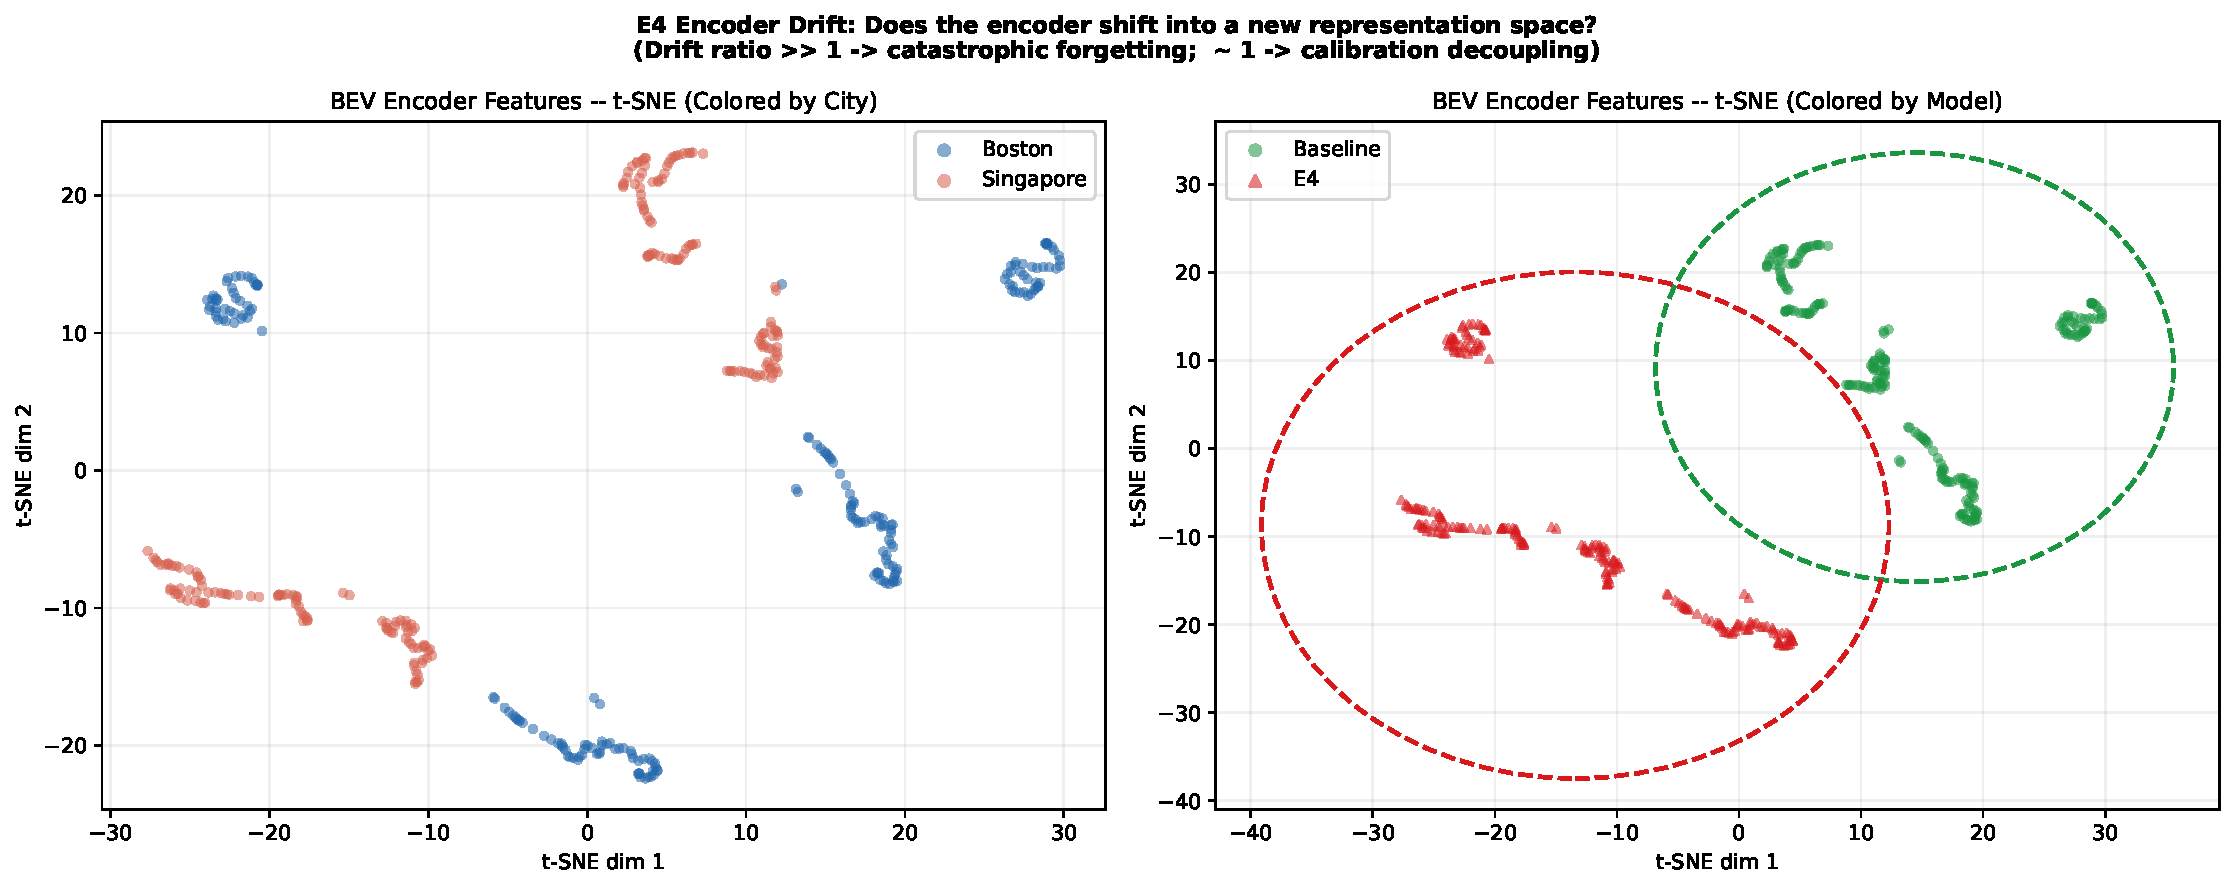
\includegraphics[width=0.9\linewidth]{../figures/tsne_encoder_drift.pdf}
  \caption{t-SNE of BEV encoder features (200 Boston, 200 Singapore frames).
    Partial separation is visible, confirming the feature space is not
    fully city-agnostic after the BEV encoder's directional normalization.
    \emph{Note: t-SNE is a visualization tool; pairwise distances in the 2D
    embedding do not reliably reflect distances in the original 256-D space.}
    The quantitative structural evidence is reported in \cref{tab:drift}
    (cross-city cosine distance $1.133\times$ within-city).}
  \label{fig:tsne}
\end{figure}

t-SNE intentionally does not preserve global distances or density faithfully in
two dimensions; pairwise distances in the projection are therefore not a valid
structural metric.
The \emph{quantitative} evidence for persistent separation is the cosine distance
ratio from \cref{tab:drift}: cross-city \texttt{bev\_embed} cosine distance is
$1.133\times$ the within-Boston baseline ($0.110$ vs.\ $0.097$ in the original
feature space).
The t-SNE figure serves as qualitative corroboration of that finding.
Together, these observations support the ``calibration decoupling'' hypothesis:
the BEV encoder normalizes gross directional appearance differences but does not
fully collapse the city-level distributional separation, leaving the detection head
seeing a measurably different feature distribution for Singapore traffic.

\subsection{DAv2 Depth Feature Stability}

We verify that DAv2 ViT-S features are domain-stable using a 100-frame stability
analysis (50 Boston, 50 Singapore, CAM\_FRONT, seed 42).
\Cref{tab:dav2} summarizes the key statistics.

\begin{table}[h]
\centering
\caption{DAv2 ViT-S feature statistics across cities (50 frames each).
  Cohen's $d < 0.2$ indicates negligible difference.}
\label{tab:dav2}
\setlength{\tabcolsep}{4pt}
\begin{tabular}{@{}lcccc@{}}
\toprule
Statistic & Boston & Singapore & Cohen's $d$ & Interpretation \\
\midrule
log-std (depth scale) & $1.000$ & $1.000$ & $0.09$ & \textbf{Identical} \\
grad\_mean (edge sharpness) & $0.054$ & $0.077$ & $0.69$ & Moderate \\
grad\_p90 & $0.018$ & $0.039$ & $1.05$ & Large \\
edge\_corr & $0.228$ & $0.152$ & $-0.90$ & Large \\
\bottomrule
\end{tabular}
\end{table}

Critically, the depth scale distribution is effectively identical
(Cohen's $d = 0.09$), confirming that DAv2's monocular depth scale is
domain-invariant across cities.
The gradient and edge statistics differ more substantially, reflecting different
scene structure (Singapore's more uniform street grid vs.\ Boston's denser urban
fabric) rather than model instability.
The geometric prior that DAv2 encodes is valid in both cities.

%% ────────────────────────────────────────────────────────────────────────────
\section{Adapter Ablation: Why Injection Fails}
\label{sec:ablation}

\subsection{Architecture}
\label{sec:arch}

\begin{figure}[h]
  \centering
  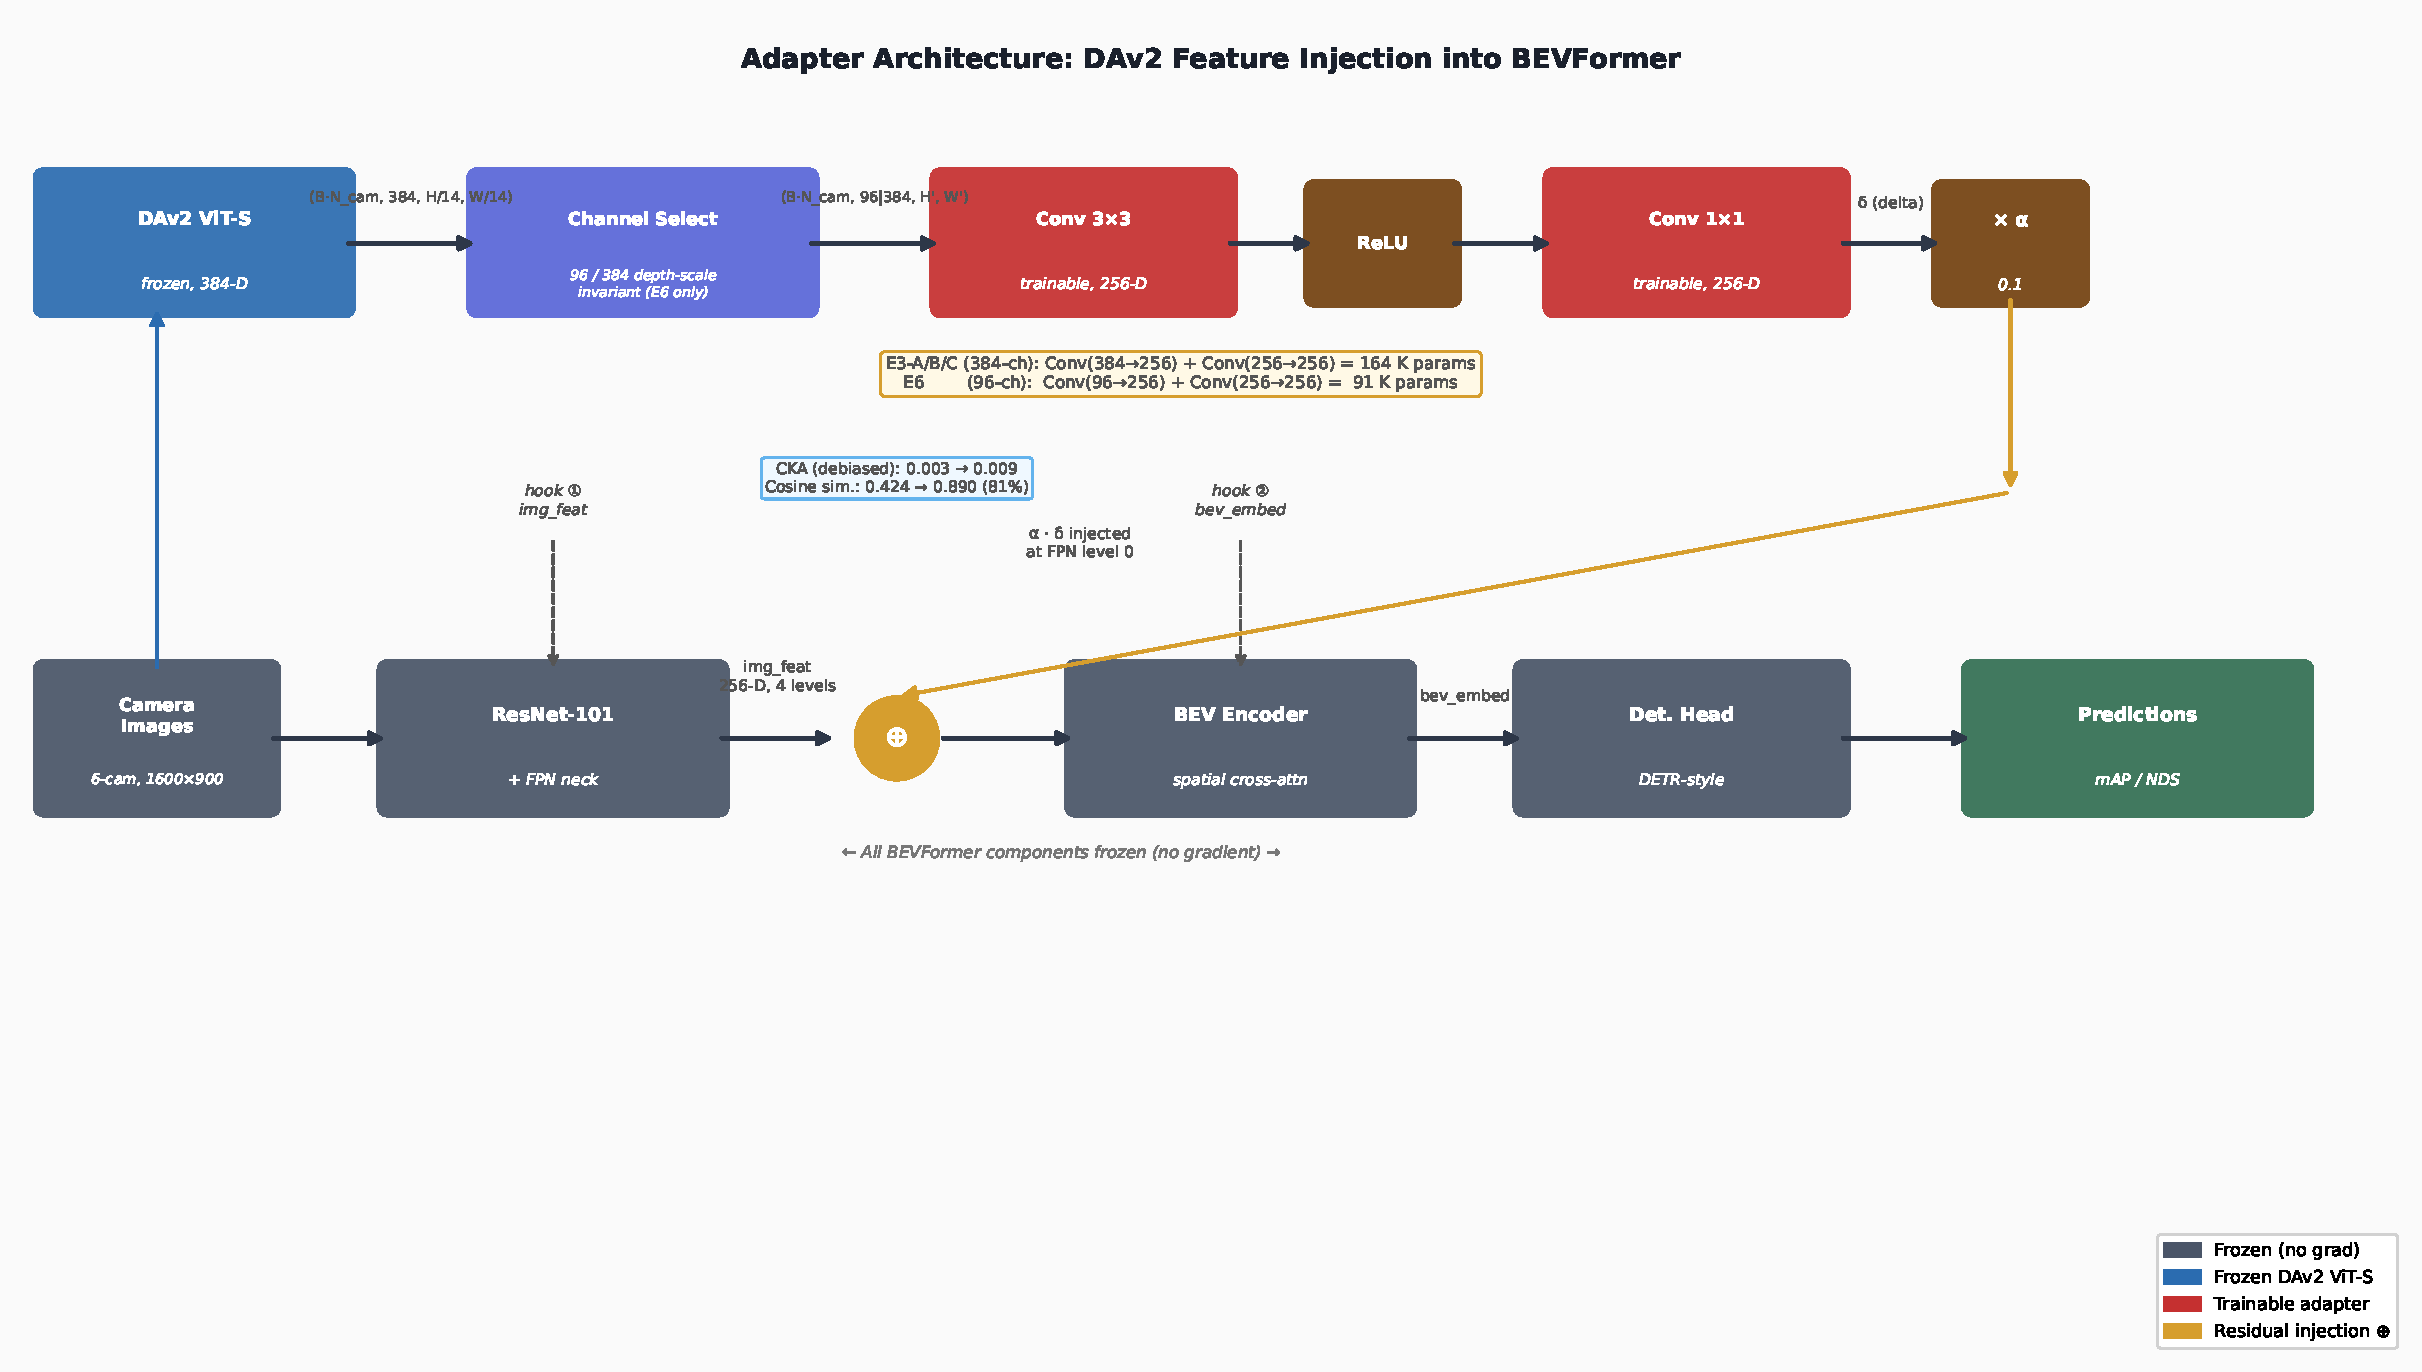
\includegraphics[width=\linewidth]{../figures/adapter_schematic.pdf}
  \caption{Adapter architecture. DAv2 ViT-S features (384-D or 96-D for E6)
    are processed by two convolutional layers (trainable) and injected as a
    scaled residual at FPN level~0, immediately before the BEV encoder.
    All BEVFormer components are frozen throughout.}
  \label{fig:adapter}
\end{figure}

We inject DAv2 features into BEVFormer at the finest FPN scale (level~0, stride~8),
immediately before the BEV encoder processes image features.
The adapter consists of two convolutional layers:
\begin{equation}
  \delta = \text{Conv}_{1\times1}(\text{ReLU}(\text{Conv}_{3\times3}(f_\text{DAv2})))
  \qquad
  \hat{f}_\text{img} = f_\text{img} + \alpha \cdot \delta
\end{equation}
where $f_\text{DAv2} \in \mathbb{R}^{B \times 384 \times H \times W}$ are DAv2 encoder
features (bilinearly resized to match FPN resolution), $f_\text{img}$ are FPN features,
$\alpha$ is the residual scale, and $\delta \in \mathbb{R}^{B \times 256 \times H \times W}$.
Both convolutional layers are initialized with near-zero weights (std $= 0.001$).
The adapter has $164$K trainable parameters.
The DAv2 ViT-S encoder ($21$M parameters) is frozen throughout.

\subsection{Experimental Results}

\cref{tab:ablation} presents the six adapter configurations.
E3-A, E3-B, and E3-C are trained on 2{,}000 Boston training samples for 4 epochs,
starting from the pretrained baseline checkpoint.
E4 uses the same Boston subset but unfreezes the BEV encoder.
E5 trains on all 2{,}929 Singapore frames using pseudo-labels generated by the frozen
baseline model.
E6 is identical to E3-B ($\alpha = 0.1$, Boston training subset) except the adapter's
first convolution takes only the 96 depth-scale-invariant DAv2 channels
(selected by correlation with log-depth standard deviation; \cref{sec:gap} §4.4)
instead of all 384 channels, reducing trainable parameters from 164\,K to 91\,K.

\begin{table*}[t]
\centering
\caption{Adapter ablation results. All models start from the frozen BEVFormer-Base
  baseline. Singapore mAP/NDS evaluated on the 2{,}929-sample Singapore split.
  ``Identical'' denotes match to baseline at four decimal places.
  E5 uses target-domain pseudo-labels ($\tau=0.3$, 50{,}134 boxes from the frozen baseline)
  and trains only the adapter weights; all four epochs degrade vs.\ baseline.
  E6 uses only 96 depth-scale-invariant DAv2 channels; Singapore results identical to
  baseline, confirming the zero-output local optimum is independent of channel selection.
  $^{\star}$E4 Singapore values obtained by running the epoch-4 checkpoint on the
  Singapore split after training; catastrophic degradation on the full validation
  (NDS $0.500 \to 0.331$) is driven by head calibration collapse visible here too.}
\label{tab:ablation}
\setlength{\tabcolsep}{6pt}
\begin{tabular}{@{}llccccl@{}}
\toprule
Config & Modification & Full val mAP & Full val NDS
       & Singapore mAP & Singapore NDS & Root cause of failure \\
\midrule
Baseline & Frozen BEVFormer, no adapter
  & 0.405 & 0.500 & 0.367 & 0.431 & -- \\
\midrule
E3-A & $\alpha = 0.01$
  & 0.405 & 0.500 & 0.367 & 0.431 & Adapter delta $\ll 1\%$ of feature magnitude \\
E3-B & $\alpha = 0.1$
  & 0.405 & 0.500 & 0.367 & 0.431 & Adapter learns zero output (local optimum) \\
E3-C & $\alpha = 0.1$ + consistency loss
  & 0.405 & 0.500 & 0.367 & 0.431 & Augmentation $\neq$ real domain shift \\
E4   & Partial unfreeze (encoder lr $= 10^{-5}$)
  & 0.373 & 0.331 & 0.307$^{\star}$ & 0.274$^{\star}$ & Head calibration broken by encoder drift \\
\midrule
E5   & Pseudo-label adapt.\ (Singapore, score $>0.3$)
  & -- & -- & 0.360 & 0.422 & Circular optimization (pseudo-labels encode model bias) \\
\midrule
E6   & 96-ch.\ depth-scale adapter ($\alpha = 0.1$, Boston)
  & 0.405 & 0.500 & 0.367 & 0.431 & Zero-output local optimum (channel selection irrelevant) \\
\bottomrule
\end{tabular}
\end{table*}

\subsection{Mechanistic Analysis}

\paragraph{E3-A ($\alpha = 0.01$): signal too small.}
At scale $0.01$, the adapter delta contributes less than $1\%$ of the FPN feature
magnitude at initialization.
The gradient of the detection loss with respect to adapter weights through this tiny
residual is negligible.
Training produces \texttt{grad\_norm} $= 0.0000$ at every logged iteration
(verified at iterations 50, 100, 150, 500).
The adapter weight distribution does not change from initialization.
This is a scale calibration failure, not a gradient flow failure.

\paragraph{E3-B ($\alpha = 0.1$): zero-output local optimum.}
Increasing the residual scale to $0.1$ brings the adapter delta into a range where
gradients are computable, yet \texttt{grad\_norm} $= 0.0000$ persists throughout
training.
The explanation is a local optimum: the frozen BEVFormer is already minimized for
the Boston detection objective.
Any non-zero adapter output perturbs the FPN features away from the values the frozen
encoder was pre-trained to process, increasing the Boston detection loss.
The gradient therefore points toward $\delta \to 0$ regardless of initialization,
and the near-zero initialization ensures the optimizer converges there immediately.
This is a fundamental consequence of training on source-domain data alone: the
optimal adapter under Boston supervision is the identity (zero output).

\paragraph{E3-C ($\alpha = 0.1$ + consistency loss): wrong supervision signal.}
We add a consistency loss $\mathcal{L}_\text{cons} = \|\hat{f}(I) - \hat{f}(\tilde{I})\|^2$,
where $\tilde{I}$ is a ColorJitter-augmented version of the input $I$.
The intuition is to encourage DAv2 features to be invariant to appearance changes.
The loss remains flat at $2.4$ throughout training.
Two failure modes compound: (i)~Boston photometric augmentation does not approximate
the real Boston$\to$Singapore appearance shift (different road geometry, vegetation,
building density), so the model is not supervised toward the correct target distribution;
(ii)~even if the augmentation were accurate, consistency with the augmented input
does not supervise the adapter to improve \emph{detection}, only to be self-consistent
across augmentations.

\paragraph{E4 (partial unfreeze, encoder lr $= 10^{-5}$): head calibration fails.}
Unfreezing the BEV encoder with a small learning rate resolves the zero-gradient
problem: \texttt{grad\_norm} is $13$--$30$ at early iterations and the training loss
decreases steadily.
However, the full validation NDS collapses from $0.500$ to $0.331$ ($-34\%$) after
4 epochs on 2{,}000 Boston samples.
The per-error breakdown shows mAOE degrading from $0.32$ to $1.22$ radians (effectively
random orientation) and mASE from $0.28$ to $0.55$.
Running the epoch-4 checkpoint on the Singapore split yields mAP $0.307$ / NDS $0.274$
--- worse than both the baseline and E3-B --- confirming that the degradation is
not a Boston-only artefact but a catastrophic collapse across both cities.
The encoder learns new representations to accommodate the injected DAv2 features,
but the frozen detection head, calibrated to the original encoder's output space,
cannot interpret these new representations for fine-grained attribute prediction.
With 2{,}000 training samples, the encoder drifts faster than the head can recalibrate
--- in fact, the head is frozen and cannot recalibrate at all.

\paragraph{E5 (pseudo-label adaptation): self-referential supervision.}
E3-B established that Boston supervision alone is insufficient because it drives the
adapter to zero output.
E5 directly addresses this by providing target-domain detection supervision:
the frozen BEVFormer is first run on all 2{,}929 Singapore validation frames to
generate pseudo-labels.
We use score threshold $\tau = 0.3$ --- a permissive threshold that retains
$50{,}134$ boxes ($17.1$/frame).
A permissive threshold is appropriate here because the goal is to provide gradient
signal across a wide range of Singapore detections, not to filter to high-purity
positive examples; raising to $\tau = 0.5$ reduces the count to $35{,}975$ boxes
($12.3$/frame, $-28\%$) and $\tau = 0.7$ to $28{,}799$ ($9.8$/frame, $-43\%$)
--- reductions that would decrease coverage without addressing the structural failure
identified below, since the self-referential mechanism operates regardless of threshold.
The adapter is then trained on Singapore pseudo-labeled frames with the BEVFormer
backbone and detection head frozen, so only the adapter weights receive gradients.

Unlike E3, \texttt{grad\_norm} is non-zero throughout training ($0.02 \to 0.13$
over the first 150 iterations), confirming that pseudo-label detection loss provides
a non-trivial gradient signal.
However, the Singapore evaluation at each epoch shows:
\emph{all four epochs are worse than the frozen baseline} (best epoch: mAP $0.360$,
NDS $0.422$; baseline: mAP $0.367$, NDS $0.431$), with performance monotonically
decreasing over training.

The failure mechanism is \textbf{self-referential supervision}.
The pseudo-labels are generated by the same frozen model that the adapter wraps.
Training the adapter to minimize detection loss on these pseudo-labels is equivalent
to asking the adapter to bring image features closer to the specific representations
that the frozen backbone and head were pre-trained to process on Boston.
This is the opposite of domain adaptation: the gradient pushes FPN features
toward the Boston-optimal manifold.
The adapter reinforces existing source biases rather than correcting for city shift.
This pattern --- degradation despite valid gradient flow --- is analogous to the
degenerate pseudo-labeling mode analyzed for 2D source-free domain adaptation in
SHOT~\cite{liang2021shot}; the distinction here is the structured 3D box regression
setting, where pseudo-labels encode box size and orientation priors internalized from
Boston, making self-referential collapse particularly severe.
This failure mode requires a supervision signal that is genuinely \emph{independent}
of the model being adapted: labels from an independent oracle, cross-modal geometric
consistency, or structure-from-motion depth supervision.

\noindent\textbf{Limitation note.}
E5 trains and evaluates on the same 2{,}929 Singapore frames.
Because E5 performance declines monotonically across all four epochs and never exceeds
the frozen baseline, this train/test overlap does not affect our conclusion:
adaptation with self-generated pseudo-labels is harmful regardless of which frames
are used for evaluation.

\paragraph{E6 (96-channel depth-scale adapter): channel selection is irrelevant.}
E6 is identical to E3-B except the adapter's first convolution receives only the 96
depth-scale-invariant DAv2 channels (25\% of the total 384 channels, selected by
$|r|$ with log-depth standard deviation across 100 calibration frames).
The adapter has 91\,K trainable parameters vs.\ 164\,K for E3-B.
\texttt{grad\_norm} is $0.0000$ at every logged iteration across all four epochs ---
identical to E3-B.
This directly confirms that the zero-output local optimum is a property of the
\emph{supervision signal} (Boston detection loss), not the input channels.
Restricting to geometrically stable channels does not help when the loss gradient
systematically drives the adapter toward zero output regardless of what it processes.

\subsection{Implications for Future Work}

The four failures define the design space for any successful frozen-adapter approach:

\begin{enumerate}
  \item \textbf{Target-domain detection signal is necessary but not sufficient.}
    E3-A, E3-B, and E6 show that Boston detection loss alone drives any adapter to
    zero output --- this holds whether injecting all 384 DAv2 channels (E3-B) or
    only the 96 depth-scale-invariant channels (E6).
    E5 shows that even with target-domain pseudo-label supervision, performance degrades
    because the pseudo-labels are generated by the same frozen model, creating a circular
    optimization that reinforces existing biases.
    A genuinely independent supervision signal --- labels from an oracle, a cross-modal
    consistency loss, or structure-from-motion depth supervision --- is required.

  \item \textbf{Appearance augmentation must approximate the real shift.}
    E3-C shows that ColorJitter does not approximate Boston$\to$Singapore shift.
    More structured augmentations (style transfer, diffusion-based domain translation)
    might provide a more accurate proxy signal, but only if they are calibrated to
    the specific target city.

  \item \textbf{Joint adaptation requires sufficient data and a flexible head.}
    E4 shows that partial encoder unfreezing can produce gradients, but without
    enough data to simultaneously update the encoder and recalibrate the head, the
    system breaks.
    A detection head that can adapt jointly with the encoder --- or a larger training
    set on both cities --- is a prerequisite for the partial unfreeze strategy to work.

  \item \textbf{The BEV encoder normalizes appearance but not structural geometry.}
    The \texttt{bev\_embed} cosine distance ratio ($1.133\times$, 95\,\% CI $[1.101,\
    1.167]$, two-sample permutation $p < 0.001$; see \cref{sec:repr} for procedure)
    and debiased CKA of $0.009$ (95\,\% CI $[0.004,\ 0.014]$)
    both confirm that city-level structural separation persists in the original
    high-dimensional feature space despite $81\%$ cosine normalization toward unity.
    This structural separation is the proximate cause of the detection gap and is the
    signal that any successful adapter must eliminate.
\end{enumerate}

%% ────────────────────────────────────────────────────────────────────────────
\section{Conclusion}
\label{sec:conclusion}

We have established a controlled Boston$\to$Singapore evaluation protocol on nuScenes
and measured a $-5.84$ mAP / $-9.25$ NDS domain gap under city-level shift with
identical hardware.
Layer-wise representation analysis shows cosine similarity rises from $0.424$ to
$0.890$ ($81\%$ per-frame normalization) while debiased CKA values are near zero in
all comparison types (within-city and cross-city alike), indicating high frame-level
scene heterogeneity dominates structural geometry; the \texttt{bev\_embed} cosine distance ratio ($1.133\times$ cross-city
vs.\ within-Boston, 95\,\% CI $[1.101,\ 1.167]$, $p < 0.001$)
provides the primary quantitative evidence that city-level structural separation
persists at the BEV encoder output; t-SNE corroborates this qualitatively.
DAv2 depth-scale features are domain-invariant across cities (Cohen's $d = 0.09$),
validating them as a geometric prior.

Our systematic ablation of \textbf{six} adapter designs (E3-A through E6) shows each
fails for a principled, distinct reason: signal magnitude collapse, zero-output local
optimum under source-domain supervision (replicated in E6 with 96-channel depth-scale
injection, confirming the failure is in the supervision signal not the channel
selection), mismatched augmentation supervision, head-calibration breakdown under
partial unfreeze, and circular pseudo-label optimization.
The E5 result is especially instructive: gradient flow is present yet performance
degrades, because the pseudo-label signal encodes model biases rather than correcting
for city-level shift.

These findings suggest that successful camera BEV domain generalization without
target-domain data will require either genuinely independent supervision signals
(oracle labels, cross-modal geometric consistency, or structure-from-motion depth),
or architectural designs that allow joint head and encoder adaptation with
low-data efficiency.
The evaluation protocol, city-split PKL files, and all experiment configs are
released to provide a reproducible benchmark for future work.

%% ────────────────────────────────────────────────────────────────────────────
\bibliographystyle{IEEEtran}
\bibliography{refs}

% Key references to add to refs.bib:
% BEVFormer: Li et al., ECCV 2022
% BEVDepth: Li et al., AAAI 2023
% StreamPETR: Wang et al., ICCV 2023
% nuScenes: Caesar et al., CVPR 2020
% DA-BEV: Jiang et al., ECCV 2024
% DAv2: Yang et al., NeurIPS 2024
% ST3D: Yang et al., CVPR 2021
% MLC-Net: Luo et al., CVPR 2021
% TENT: Wang et al., ICLR 2021
% SHOT: Liang et al., ICML 2021
% TTT: Sun et al., ICML 2020

\end{document}
